\chapter{CSC-LISTA: the architecture}\label{ch:csc_lista}

This chapter goes through the network piece by piece, and checks each piece against Eq.~20.

\section{The equation}

Eq.~20 of Liu et al., for layer $k$ and atom $m$:
\begin{equation}
x_m^{(k+1)} = \soft_{\theta^{(k)}}\!\left( x_m^{(k)} - \big(w_m^{(k)}\big)' *
\Big( \sum_{\bar m=1}^{M} d_{\bar m} * x_{\bar m}^{(k)} - b \Big) \right). \tag{Liu et al., Eq.~20}
\end{equation}

Read it from the inside out, in plain words:

\begin{enumerate}
\item $\sum d_{\bar m}*x_{\bar m}$: blur the current codes back into a predicted measurement.
\item Subtract $b$: this is the mismatch, also called the \textbf{residual}.
\item $(w_m)'*$: pass the residual through a learned filter, once per atom. This turns one image of
mismatch into 32 maps of correction.
\item Subtract the correction from $x_m$.
\item $\soft_\theta$: shrink, so that small values become zero.
\end{enumerate}

Compare it with ISTA. There, $(w_m)'$ is fixed at $d_m'/L$. So the entire change in Eq.~20 is that
\emph{each layer gets to learn its own correction filter and its own threshold}.

\section{Everything in one picture}

\begin{figure}[H]
\centering
\begin{tikzpicture}[node distance=7mm and 9mm]
\node[fixed] (x) {Codes $x^{(k)}$\\ 32 maps};
\node[fixed,right=14mm of x] (D) {Blur and stamp\\ $\sum_m d_m*x_m$\\ \footnotesize fixed};
\node[block,right=14mm of D] (r) {Residual\\ mask $\cdot\,(\cdot-b)$};
\node[learned,below=of r] (w) {Correction filters\\ $(w_m^{(k)})'*$\\ \footnotesize learned, 32 of 155 px};
\node[block,left=14mm of w] (sub) {$x^{(k)} -$ correction};
\node[learned,left=14mm of sub] (s) {Shrink $\soft_{\theta^{(k)}}$\\ \footnotesize one learned $\theta$};
\node[fixed,below=of s] (next) {Codes $x^{(k+1)}$};
\node[fixed,above=6mm of r] (b) {Input $b$};
\draw[flow] (x)--(D); \draw[flow] (D)--(r); \draw[flow] (b)--(r);
\draw[flow] (r)--(w); \draw[flow] (w)--(sub); \draw[flow] (sub)--(s); \draw[flow] (s)--(next);
\draw[dashflow] (x.south) |- ($(sub.north)+(0,3.5mm)$) -- (sub.north);
\end{tikzpicture}
\caption{One CSC-LISTA layer. Orange boxes are learned. Grey boxes are fixed. After the final layer,
the output field is $\sum_m g_m * x_m^{(K)}$.}
\label{fig:layer}
\end{figure}

\section{The sizes of everything}

\begin{center}
\begin{tabular}{llp{6.7cm}}
\toprule
Object & Shape & Meaning \\
\midrule
\code{b} & $[B, N, N]$ & Batch of padded input images \\
\code{x} & $[B, 32, N, N]$ & 32 code maps per image, one per atom \\
\code{atoms} & $[32, 75, 75]$ & Sharp dictionary $g_m$, 7.5\um\ wide, fixed \\
\code{w} & $[K, 32, 155, 155]$ & Learned filters, 15.5\um\ wide \\
\code{theta} & $[K]$ & One threshold per layer \\
\bottomrule
\end{tabular}
\end{center}

During training $N=768$, which is a 512 pixel crop plus 128 pixels of padding on each side. On a
full image $N=1656$. The same weights work at both sizes, because the network is convolutional.

The parameter count comes straight from these shapes:
\begin{equation}
K \times (155^2 \times 32) + K .
\end{equation}
This gives 12,300,816 at 16 layers, 24,601,632 at 32, and 49,203,264 at 64. Those numbers match
the saved run files.

\section{The code, line by line}

\subsection*{The operator: convolving with many filters using FFTs}

A 75 pixel filter convolved directly on a $768\times768$ image would be far too slow, and the blur
$h$ is defined in Fourier space anyway. So every convolution is done as a multiplication of spectra.
\code{Operator} wraps this.

\begin{code*}{csc_lista.py}
class Operator:
    """A convolutional dictionary, optionally followed by the standoff filter h.

    Spectra are built on demand and `chunk` filters at a time, so a full image
    never holds every filter spectrum in memory at once.
    """

    def __init__(self, filters, h=None, chunk=None):
        self.filters, self.h = filters, h
        self.chunk = chunk or filters.shape[0]

    def spectra(self, n):
        for first in range(0, self.filters.shape[0], self.chunk):
            part = centred_rfft(self.filters[first:first + self.chunk], n)
            yield first, part if self.h is None else part * self.h
\end{code*}

Look at the last line. If \code{h} is given, each filter's spectrum is multiplied by $h$. \textbf{That
single multiplication is $d_m=h*g_m$.} The same class is the sharp dictionary $G$ when \code{h} is
\code{None}, and the blurred dictionary $D$ when \code{h} is set.

\begin{code*}{csc_lista.py}
    def forward(self, x):
        """sum_m filter_m * x_m for maps [B, M, N, N]; returns [B, N, N]."""
        n = x.shape[-1]
        total = 0
        for first, part in self.spectra(n):
            total = total + (torch.fft.rfft2(x[:, first:first + part.shape[0]]) * part).sum(1)
        return torch.fft.irfft2(total, s=(n, n))

    def adjoint(self, residual):
        """filter_m' * residual, the transpose of forward, for [B, N, N] input."""
        n = residual.shape[-1]
        spectrum = torch.fft.rfft2(residual)[:, None]
        return torch.cat([torch.fft.irfft2(spectrum * part.conj(), s=(n, n))
                          for _, part in self.spectra(n)], 1)
\end{code*}

\code{forward} is $\sum_m f_m*x_m$: many maps go in, one image comes out. \code{adjoint} goes the
other way: one image goes in, 32 maps come out.

\begin{keyidea}[Why \texttt{part.conj()} is the 180-degree rotation]
Eq.~20 needs $(w_m)'$, the filter rotated by 180 degrees. For a real filter, rotating by 180 degrees in
space is the same as taking the complex conjugate in Fourier space. So \code{part.conj()} is exactly the prime in
the equation. A unit test confirms that \code{forward} and \code{adjoint} are true transposes.
\end{keyidea}

\subsection*{The largest eigenvalue $L$}

\begin{code*}{csc_lista.py}
    def bound(self, n):
        """Largest eigenvalue of D D^T on an n-square canvas."""
        return float(sum((part.abs() ** 2).sum(0) for _, part in self.spectra(n)).max())
\end{code*}

In Fourier space the operator splits into small independent pieces, one per frequency. So the
largest eigenvalue is simply the largest value of $\sum_m|D_m(f)|^2$ over all frequencies. For our
dictionary, $L\approx77{,}633$.

\subsection*{The starting point: the network begins as ISTA}

\begin{code*}{csc_lista.py}
        h = transfer(canvas, dx, dz, atoms.dtype, atoms.device)
        operator = Operator(atoms, h, chunk)
        step = 1 / operator.bound(canvas)
        self.bound_value = 1 / step
        # ISTA start: w = d / L, truncated to the filter support.
        rows = []
        for first, part in operator.spectra(canvas):
            full = torch.roll(torch.fft.irfft2(part, s=(canvas, canvas)),
                              (width // 2, width // 2), (-2, -1))
            rows.append(full[..., :width, :width] * step)
        self.w = nn.Parameter(torch.cat(rows)[None].repeat(layers, 1, 1, 1))
        self.theta = nn.Parameter(torch.full((layers,), lam * step, dtype=atoms.dtype,
                                             device=atoms.device))
\end{code*}

Each $w$ starts as $d_m/L$, cut to 155 pixels, and each threshold starts at $\lambda/L$. All layers
start identical. So before training the network \emph{is} ISTA, apart from the cut. A test confirms this: with
filters wide enough, the untrained network matches ISTA to within 2\%.

\subsection*{One layer}

Here is Eq.~20 in the code. Compare it with the equation, term by term.

\begin{code*}{csc_lista.py}
    def layer(self, x, b, k, operator, mask):
        residual = mask * (operator.forward(x) - b)
        update = x - Operator(self.w[k], chunk=self.chunk).adjoint(residual)
        return shrink(update, self.theta[k].clamp_min(0))
\end{code*}

\begin{center}
\renewcommand{\arraystretch}{1.5}
\begin{tabular}{p{5.1cm}p{9.4cm}}
\toprule
Paper & Code \\
\midrule
$\sum_{\bar m} d_{\bar m}*x_{\bar m}$ & \code{operator.forward(x)} \\
$\sum_{\bar m} d_{\bar m}*x_{\bar m} - b$ & \code{mask * (operator.forward(x) - b)} \\
$(w_m^{(k)})' * (\cdot)$ & \code{Operator(self.w[k], ...).adjoint(residual)} \\
$x_m^{(k)} - (\cdot)$ & \code{update = x - ...} \\
$\soft_{\theta^{(k)}}(\cdot)$ & \code{shrink(update, self.theta[k].clamp_min(0))} \\
Sum over $m=1\dots M$ & Handled by the tensor shapes \\
\bottomrule
\end{tabular}
\end{center}

Two small things in that code are not in the equation: the \code{mask} and the \code{clamp_min(0)}.
Both are listed in Chapter~\ref{ch:differences}.

\subsection*{All the layers, and the output}

\begin{code*}{csc_lista.py}
    def codes(self, b):
        n = b.shape[-1]
        operator, mask = self.physics(n)
        x = torch.zeros(b.shape[0], self.w.shape[1], n, n, dtype=b.dtype, device=b.device)
        y = x
        for k in range(self.layers):
            if self.use_checkpoint and self.training:
                update = checkpoint(self.layer, y, b, k, operator, mask, use_reentrant=False)
            else:
                update = self.layer(y, b, k, operator, mask)
            y = update if self.beta is None else update + self.beta[k] * (update - x)
            x = update
        return x
\end{code*}

Codes start at zero. For Eq.~20 runs \code{self.beta} is \code{None}, so \code{y} is simply the latest
\code{update}. The momentum line matters only in Chapter~\ref{ch:lfista}.

\code{checkpoint} is a memory trick. It throws away intermediate values during the forward pass and
recomputes them when needed for gradients. It does not change the result.

\begin{code*}{csc_lista.py}
    def forward(self, b):
        """b is [B, N, N], zero-padded; returns the padded output field."""
        return Operator(self.atoms, chunk=self.chunk).forward(self.codes(b))
\end{code*}

No $h$ is used here. Codes found with the blurred $D$ are stamped with the sharp $G$. The paper's
Appendix H does the matching thing: it reconstructs by ``convolving the learned feature maps with the
original dictionary''.

\section{Why the padding and the mask exist}

FFT convolution is circular: what leaves one edge reappears at the opposite edge. Also, a wire just
outside the crop still affects the field inside it. So:

\begin{enumerate}
\item The input is padded with 128 pixels of zeros.
\item Codes live on the larger canvas, so they can explain field that arrives from outside.
\item The residual is multiplied by a mask that is 1 inside the true image and 0 in the padding.
\end{enumerate}

\begin{code*}{csc_lista.py}
def window_mask(n, pad, device='cpu'):
    mask = torch.zeros(n, n, device=device)
    mask[pad:n - pad, pad:n - pad] = 1
    return mask
\end{code*}

Without the mask, the network would be told the field is truly zero in the padding, which is false. The
paper has the same concern: in its Eq.~18 the code $x_m$ is larger than the image $b$. A test confirms that
changing the padded region of the input does not change the output.

\section{What the learned filters look like}

\begin{figure}[H]
\centering
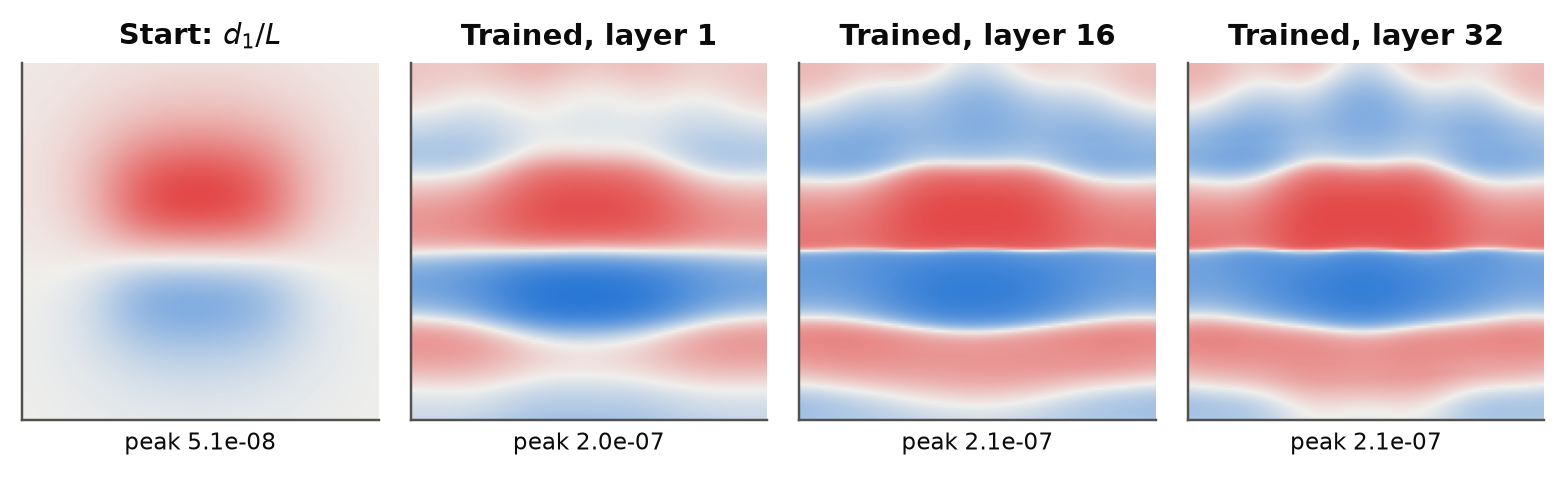
\includegraphics[width=\textwidth]{filters_w}
\caption{Filter $w_1$ for the first atom, at the start and after training, from the strict 32-layer
model at its best step. Each panel has its own colour scale. Training made the filters about four times
stronger, and added ripples.}
\label{fig:w}
\end{figure}

Figure~\ref{fig:w} shows something useful. The start is a smooth blob. After training, the filter has
alternating bands. Sign-changing ripples like that are what sharpening filters look like, since they
boost the frequencies that blur removed. For this atom, the trained filters also differ little between layers.
